\section{Configuration Dialog}
\label{sec:analyze_dialog}

Selecting an entry from the 'Analyze' menu opens the Analyze Data Source dialog, pre-configured for MLAT. \\\\

\begin{figure}[H]
  \centering
  \hspace*{-1.0cm}
    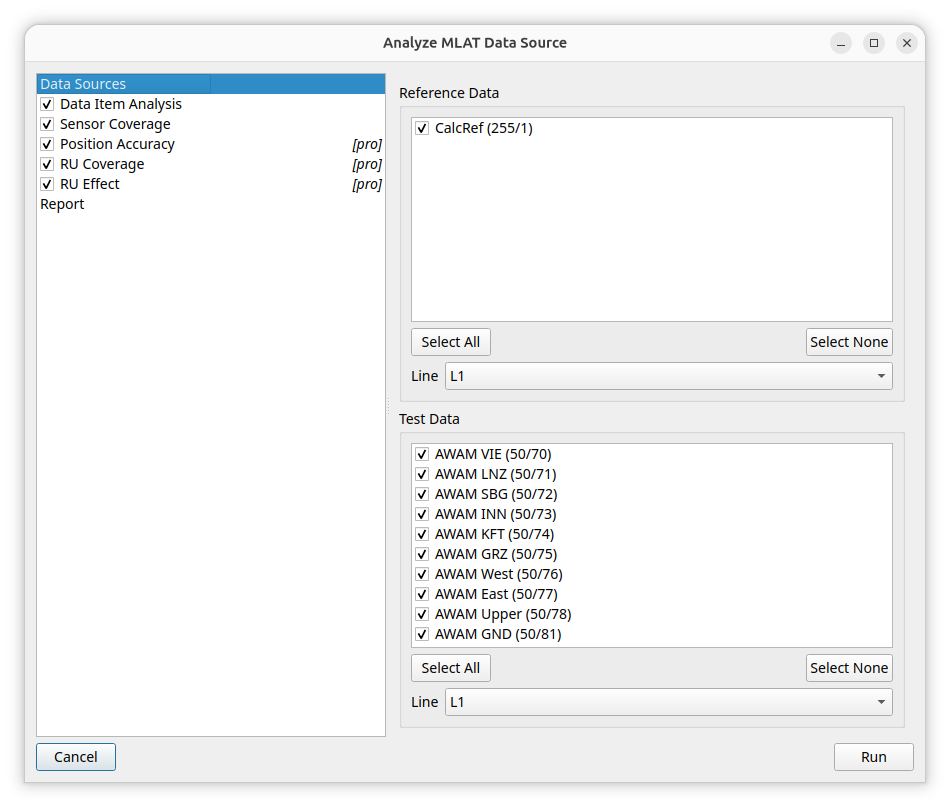
\includegraphics[width=17cm]{figures/analyze_mlat.png}
  \caption{Analyze MLAT dialog}
\end{figure}


The dialog is split into a navigation tree on the left and a stacked detail widget on the right. \\

\begin{itemize}
\item Left tree
\begin{itemize}
\item 'Data Source' node: top-level entry; selecting it shows the Data Source selection widget on the right
\item One node per available inspector, each with an active checkbox controlling whether that inspector runs
\end{itemize}
\item Right pane
\begin{itemize}
\item Shows the settings widget of the currently highlighted tree node
\item When the 'Data Source' node is selected, lists all Data Sources of the bound DSType with checkboxes
\item When an inspector node is selected, exposes the parameters specific to that inspector
\end{itemize}
\item Bottom
\begin{itemize}
\item 'Run' button: executes the enabled inspectors; performs validation first
\item 'Cancel' button: closes the dialog without running
\end{itemize}
\end{itemize}
\ \\

Inspectors whose prerequisites are not met (e.g. Pro inspectors without an active Professional license, or RU-based inspectors without CAT020 data) appear greyed out. The corresponding tooltip explains the reason the inspector cannot be selected. \\

\textcolor{red}{\textbf{[TODO: check that the screenshot above shows the current dialog, including the 'Scope Filter' box with the 'Use Evaluation Exclusions' row]}} \\

\subsection{Scope Filter}
\label{sec:analyze_scope_filter}

The 'Scope Filter' box on the 'Data Source' page restricts which target reports are used by the analysis.
It is applied when the data is loaded, so all inspectors use the same target reports. All selected constraints must be met. \\

\begin{figure}[H]
  \center
    \fbox{\parbox{0.8\textwidth}{\vspace{1.5cm}\centering \textcolor{red}{\textbf{[FIGURE TODO: 'Data Source' page of the Analyze MLAT dialog, 'Scope Filter' box with all rows visible, 'Use Evaluation Exclusions' checked, 'Limit by Sectors' checked with some sector layers selected]}}\vspace{1.5cm}}}
  \caption{Analyze dialog Scope Filter}
\end{figure}

\begin{itemize}
\item Use Ground Only: keeps only target reports on the ground
\begin{itemize}
\item On the ground: ground bit set, or ground-only target type, or ground-only Data Source (SMR)
\end{itemize}
\item Minimum Flight Level: keeps only target reports at or above the given flight level
\item Maximum Flight Level: keeps only target reports at or below the given flight level
\begin{itemize}
\item Both use the barometric altitude, target reports without an altitude are kept
\end{itemize}
\item Use Evaluation Exclusions: leaves out the data excluded in the Evaluation
\begin{itemize}
\item Targets not used in the Evaluation, with their reference and test target reports
\item Target reports in the excluded time windows of a target
\item If the Evaluation timestamp filter is used: target reports outside the timestamp begin and end, and in the global excluded time windows
\item Target reports without a target (unassociated) are only checked against the global time constraints
\item A reference period ends at an excluded time window and starts again after it, as in the Evaluation
\item Excluded requirements are only used by the Evaluation and are ignored
\end{itemize}
\item Limit by Sectors: keeps only target reports inside at least one of the selected sector layers
\begin{itemize}
\item Same inside test as the Evaluation, including the altitude limits and exclusion sectors
\item 'Run' is disabled when no sector layer is selected
\end{itemize}
\end{itemize}
\ \\

The Evaluation exclusions are defined in the \nameref{sec:targets} tool of the Flight Deck:

\begin{itemize}
\item Use flags: \nameref{sec:ui_eval_usage}, also with the \nameref{sec:ui_target_filtering} dialog, e.g. to leave out certain target types
\item Global time constraints: \nameref{sec:ui_eval_global_excl_tw}
\item Target time windows: \nameref{sec:ui_eval_target_excl_tw}
\end{itemize}
\ \\


\includegraphics[width=0.5cm]{../../data/icons/hint.png} \textbf{Please note that the exclusions are read when the analysis is run.
If they are changed later, the analysis report has to be updated to use the changed exclusions.} \\

